% Options for packages loaded elsewhere
\PassOptionsToPackage{unicode}{hyperref}
\PassOptionsToPackage{hyphens}{url}
%
\documentclass[
]{article}
\usepackage{amsmath,amssymb}
\usepackage{lmodern}
\usepackage{ifxetex,ifluatex}
\ifnum 0\ifxetex 1\fi\ifluatex 1\fi=0 % if pdftex
  \usepackage[T1]{fontenc}
  \usepackage[utf8]{inputenc}
  \usepackage{textcomp} % provide euro and other symbols
\else % if luatex or xetex
  \usepackage{unicode-math}
  \defaultfontfeatures{Scale=MatchLowercase}
  \defaultfontfeatures[\rmfamily]{Ligatures=TeX,Scale=1}
\fi
% Use upquote if available, for straight quotes in verbatim environments
\IfFileExists{upquote.sty}{\usepackage{upquote}}{}
\IfFileExists{microtype.sty}{% use microtype if available
  \usepackage[]{microtype}
  \UseMicrotypeSet[protrusion]{basicmath} % disable protrusion for tt fonts
}{}
\makeatletter
\@ifundefined{KOMAClassName}{% if non-KOMA class
  \IfFileExists{parskip.sty}{%
    \usepackage{parskip}
  }{% else
    \setlength{\parindent}{0pt}
    \setlength{\parskip}{6pt plus 2pt minus 1pt}}
}{% if KOMA class
  \KOMAoptions{parskip=half}}
\makeatother
\usepackage{xcolor}
\IfFileExists{xurl.sty}{\usepackage{xurl}}{} % add URL line breaks if available
\IfFileExists{bookmark.sty}{\usepackage{bookmark}}{\usepackage{hyperref}}
\hypersetup{
  pdftitle={Stat 230 HW 4},
  pdfauthor={Name: Victor Huang},
  hidelinks,
  pdfcreator={LaTeX via pandoc}}
\urlstyle{same} % disable monospaced font for URLs
\usepackage[margin=1in]{geometry}
\usepackage{color}
\usepackage{fancyvrb}
\newcommand{\VerbBar}{|}
\newcommand{\VERB}{\Verb[commandchars=\\\{\}]}
\DefineVerbatimEnvironment{Highlighting}{Verbatim}{commandchars=\\\{\}}
% Add ',fontsize=\small' for more characters per line
\usepackage{framed}
\definecolor{shadecolor}{RGB}{248,248,248}
\newenvironment{Shaded}{\begin{snugshade}}{\end{snugshade}}
\newcommand{\AlertTok}[1]{\textcolor[rgb]{0.94,0.16,0.16}{#1}}
\newcommand{\AnnotationTok}[1]{\textcolor[rgb]{0.56,0.35,0.01}{\textbf{\textit{#1}}}}
\newcommand{\AttributeTok}[1]{\textcolor[rgb]{0.77,0.63,0.00}{#1}}
\newcommand{\BaseNTok}[1]{\textcolor[rgb]{0.00,0.00,0.81}{#1}}
\newcommand{\BuiltInTok}[1]{#1}
\newcommand{\CharTok}[1]{\textcolor[rgb]{0.31,0.60,0.02}{#1}}
\newcommand{\CommentTok}[1]{\textcolor[rgb]{0.56,0.35,0.01}{\textit{#1}}}
\newcommand{\CommentVarTok}[1]{\textcolor[rgb]{0.56,0.35,0.01}{\textbf{\textit{#1}}}}
\newcommand{\ConstantTok}[1]{\textcolor[rgb]{0.00,0.00,0.00}{#1}}
\newcommand{\ControlFlowTok}[1]{\textcolor[rgb]{0.13,0.29,0.53}{\textbf{#1}}}
\newcommand{\DataTypeTok}[1]{\textcolor[rgb]{0.13,0.29,0.53}{#1}}
\newcommand{\DecValTok}[1]{\textcolor[rgb]{0.00,0.00,0.81}{#1}}
\newcommand{\DocumentationTok}[1]{\textcolor[rgb]{0.56,0.35,0.01}{\textbf{\textit{#1}}}}
\newcommand{\ErrorTok}[1]{\textcolor[rgb]{0.64,0.00,0.00}{\textbf{#1}}}
\newcommand{\ExtensionTok}[1]{#1}
\newcommand{\FloatTok}[1]{\textcolor[rgb]{0.00,0.00,0.81}{#1}}
\newcommand{\FunctionTok}[1]{\textcolor[rgb]{0.00,0.00,0.00}{#1}}
\newcommand{\ImportTok}[1]{#1}
\newcommand{\InformationTok}[1]{\textcolor[rgb]{0.56,0.35,0.01}{\textbf{\textit{#1}}}}
\newcommand{\KeywordTok}[1]{\textcolor[rgb]{0.13,0.29,0.53}{\textbf{#1}}}
\newcommand{\NormalTok}[1]{#1}
\newcommand{\OperatorTok}[1]{\textcolor[rgb]{0.81,0.36,0.00}{\textbf{#1}}}
\newcommand{\OtherTok}[1]{\textcolor[rgb]{0.56,0.35,0.01}{#1}}
\newcommand{\PreprocessorTok}[1]{\textcolor[rgb]{0.56,0.35,0.01}{\textit{#1}}}
\newcommand{\RegionMarkerTok}[1]{#1}
\newcommand{\SpecialCharTok}[1]{\textcolor[rgb]{0.00,0.00,0.00}{#1}}
\newcommand{\SpecialStringTok}[1]{\textcolor[rgb]{0.31,0.60,0.02}{#1}}
\newcommand{\StringTok}[1]{\textcolor[rgb]{0.31,0.60,0.02}{#1}}
\newcommand{\VariableTok}[1]{\textcolor[rgb]{0.00,0.00,0.00}{#1}}
\newcommand{\VerbatimStringTok}[1]{\textcolor[rgb]{0.31,0.60,0.02}{#1}}
\newcommand{\WarningTok}[1]{\textcolor[rgb]{0.56,0.35,0.01}{\textbf{\textit{#1}}}}
\usepackage{longtable,booktabs,array}
\usepackage{calc} % for calculating minipage widths
% Correct order of tables after \paragraph or \subparagraph
\usepackage{etoolbox}
\makeatletter
\patchcmd\longtable{\par}{\if@noskipsec\mbox{}\fi\par}{}{}
\makeatother
% Allow footnotes in longtable head/foot
\IfFileExists{footnotehyper.sty}{\usepackage{footnotehyper}}{\usepackage{footnote}}
\makesavenoteenv{longtable}
\usepackage{graphicx}
\makeatletter
\def\maxwidth{\ifdim\Gin@nat@width>\linewidth\linewidth\else\Gin@nat@width\fi}
\def\maxheight{\ifdim\Gin@nat@height>\textheight\textheight\else\Gin@nat@height\fi}
\makeatother
% Scale images if necessary, so that they will not overflow the page
% margins by default, and it is still possible to overwrite the defaults
% using explicit options in \includegraphics[width, height, ...]{}
\setkeys{Gin}{width=\maxwidth,height=\maxheight,keepaspectratio}
% Set default figure placement to htbp
\makeatletter
\def\fps@figure{htbp}
\makeatother
\setlength{\emergencystretch}{3em} % prevent overfull lines
\providecommand{\tightlist}{%
  \setlength{\itemsep}{0pt}\setlength{\parskip}{0pt}}
\setcounter{secnumdepth}{-\maxdimen} % remove section numbering
\ifluatex
  \usepackage{selnolig}  % disable illegal ligatures
\fi

\title{Stat 230 HW 4}
\author{Name: Victor Huang}
\date{}

\begin{document}
\maketitle

\hypertarget{worked-with-no-one}{%
\subsubsection{worked with: No one}\label{worked-with-no-one}}

Homework 4 is due \textbf{by 3pm Thursday, Oct.~14}. Please complete the
assignment in this Markdown document, filling in your answers and R code
below. I didn't create answer and R chunk fields like I did with
homework 1, but please fill in your answers and R code in the same
manner as hw 1. Submit a hard copy of the \textbf{compiled pdf or word
doc} either

\begin{itemize}
\tightlist
\item
  in class
\item
  in drop-in office hours
\item
  in the paper holder outside my CMC 222 office door
\end{itemize}

Tips for using Markdown with homework sets:

\begin{itemize}
\tightlist
\item
  Work through a problem by putting your R code into R chunks in this
  .Rmd. Run the R code to make sure it works, then knit the .Rmd to
  verify they work in that environment.

  \begin{itemize}
  \tightlist
  \item
    Make sure you load your data in the .Rmd and include any needed
    \texttt{library} commands.
  \end{itemize}
\item
  Feel free to edit or delete questions, instructions, or code provided
  in this file when producing your homework solution.
\item
  For your final document, you can change the output type from
  \texttt{html\_document} to \texttt{word\_document} or
  \texttt{pdf\_document}. These two to output types are better formatted
  for printing.

  \begin{itemize}
  \tightlist
  \item
    on maize: you may need to allow for pop-ups from this site
  \end{itemize}
\item
  If you want to knit to pdf while running Rstudio from your computer
  (\emph{not} from maize), you will need a LaTeX compiler installed on
  your computer. This could be \href{https://miktex.org/}{MiKTeX},
  \href{http://www.tug.org/mactex/}{MacTeX} (mac), or TinyTex. The
  latter is installed in R: first install the R package
  \texttt{tinytex}, then run the command
  \texttt{tinytex::install\_tinytex()} to install this software.

  \begin{itemize}
  \tightlist
  \item
    If you are using maize, you don't need to install anything to knit
    to pdf!
  \end{itemize}
\end{itemize}

\begin{center}\rule{0.5\linewidth}{0.5pt}\end{center}

\hypertarget{problem-1-depression-and-education-ch.-9-exercise-19-parts-a-b-and-c}{%
\subsection{Problem 1: Depression and Education: ch.~9 exercise 19 parts
(a), (b) and
(c)}\label{problem-1-depression-and-education-ch.-9-exercise-19-parts-a-b-and-c}}

\begin{itemize}
\item
  Part (c) is missing its label in my version of your textbook, if this
  is the case in your textbook, then part (c) is the question that
  follows the part (b) question.
\item
  There \textbf{is no data for this problem}. Write down a
  \emph{specific model mean function} \(\mu(Y \mid X) = \beta_0 + ...\)
  \textbf{with indicator variables for factor levels}.
\item
  \textbf{Hint:} You must carefully write a mean function for both parts
  (a) and (b). You will be using dummy variables for your categorical
  variable, so you must define what the dummy variable(s) are indicating
  (i.e.~which level are they identifying?). When trying to answer the
  questions about divergence, make sure to review the info provided for
  the problem - they are wondering if the difference in mean depression
  score for college (i) and high school only (iii) widens as people age.
\end{itemize}

\begin{enumerate}
\def\labelenumi{\alph{enumi})}
\item
  \[
  \hat \mu_{depression|HS,HSCD,CD} = \beta_{0} + \beta_{1}(HS) + \beta_{2}(HSCD) + \beta_{3}(CD)
  \] As we can see from the equation, the
  \(\beta_{3}(CD) - \beta_{1}(HS)\) would be the parameter that measures
  the diverging gap between categories (i) and (iii) with age.
\item
  \[
  \hat \mu_{depression|HS,HSCD,CD} = \beta_{0} + \beta_{1}(HS) + \beta_{1}(HSCD) + \beta_{3}(CD)= \beta_{0} + \beta_{1}(HS+HSCD) + \beta_{3}(CD)
  \] As we can see from the equation, a possible parameter would be
  \(\beta_{3}(CD) - \beta_{1}(HS + HSCD)\) would be a parameter that
  measures the diverging gap.
\item
  \[
  \hat \mu_{depresson|teen,middle,old} = \beta_{0} + \beta_{1}(teen) + \beta_{1}(middle) + \beta_{3}(old) + e
  \] Yes, by measuring the \(\beta_{1}(teen) - \beta_{3}(old)\)
  parameter we can see how age and education correlate with depression,
  thus, characteizing the divergence hypothesis.
\end{enumerate}

\begin{center}\rule{0.5\linewidth}{0.5pt}\end{center}

\hypertarget{problem-2-bat-echolocation}{%
\subsection{Problem 2: Bat
Echolocation}\label{problem-2-bat-echolocation}}

Use the data from case study 10.1.2 (\texttt{case1002}) to answer the
questions below.

\begin{Shaded}
\begin{Highlighting}[]
\SpecialCharTok{\textgreater{}} \FunctionTok{library}\NormalTok{(Sleuth3)}
\SpecialCharTok{\textgreater{}} \FunctionTok{library}\NormalTok{(dplyr)}
\SpecialCharTok{\textgreater{}} \FunctionTok{library}\NormalTok{(ggplot2)}
\SpecialCharTok{\textgreater{}} \FunctionTok{library}\NormalTok{(ggResidpanel)}
\SpecialCharTok{\textgreater{}} \FunctionTok{library}\NormalTok{(broom)}
\SpecialCharTok{\textgreater{}} \FunctionTok{library}\NormalTok{(knitr)}
\SpecialCharTok{\textgreater{}}\NormalTok{ case1002 }\OtherTok{\textless{}{-}}\NormalTok{ case1002}
\end{Highlighting}
\end{Shaded}

\hypertarget{a}{%
\subsubsection{(2a)}\label{a}}

Use R to fit the parallel regression lines model for the regression of
log energy on log mass and vertebrate type. (The same model fit in the
case study). Note that your model summary will be different from display
10.6 because the baseline Type group set by R is different than the
baseline used by the book. \textbf{Do not} change the baseline group in
R to make your results look like display 10.6.

\begin{Shaded}
\begin{Highlighting}[]
\SpecialCharTok{\textgreater{}}\NormalTok{ case1002 }\OtherTok{\textless{}{-}}\NormalTok{ case1002}
\SpecialCharTok{\textgreater{}}\NormalTok{ case1002\_lm }\OtherTok{\textless{}{-}} \FunctionTok{lm}\NormalTok{(}\FunctionTok{log}\NormalTok{(Energy) }\SpecialCharTok{\textasciitilde{}} \FunctionTok{log}\NormalTok{(Mass) }\SpecialCharTok{+}\NormalTok{ Type, }\AttributeTok{data=}\NormalTok{case1002)}
\SpecialCharTok{\textgreater{}} \FunctionTok{summary}\NormalTok{(case1002\_lm)}

\NormalTok{Call}\SpecialCharTok{:}
\FunctionTok{lm}\NormalTok{(}\AttributeTok{formula =} \FunctionTok{log}\NormalTok{(Energy) }\SpecialCharTok{\textasciitilde{}} \FunctionTok{log}\NormalTok{(Mass) }\SpecialCharTok{+}\NormalTok{ Type, }\AttributeTok{data =}\NormalTok{ case1002)}

\NormalTok{Residuals}\SpecialCharTok{:}
\NormalTok{     Min       1Q   Median       3Q      Max }
\SpecialCharTok{{-}}\FloatTok{0.23224} \SpecialCharTok{{-}}\FloatTok{0.12199} \SpecialCharTok{{-}}\FloatTok{0.03637}  \FloatTok{0.12574}  \FloatTok{0.34457} 

\NormalTok{Coefficients}\SpecialCharTok{:}
\NormalTok{                           Estimate Std. Error t value }\FunctionTok{Pr}\NormalTok{(}\SpecialCharTok{\textgreater{}}\ErrorTok{|}\NormalTok{t}\SpecialCharTok{|}\NormalTok{)    }
\NormalTok{(Intercept)                }\SpecialCharTok{{-}}\FloatTok{1.49770}    \FloatTok{0.14987}  \SpecialCharTok{{-}}\FloatTok{9.993} \FloatTok{2.77e{-}08} \SpecialCharTok{**}\ErrorTok{*}
\FunctionTok{log}\NormalTok{(Mass)                   }\FloatTok{0.81496}    \FloatTok{0.04454}  \FloatTok{18.297} \FloatTok{3.76e{-}12} \SpecialCharTok{**}\ErrorTok{*}
\NormalTok{Typenon}\SpecialCharTok{{-}}\NormalTok{echolocating bats  }\SpecialCharTok{{-}}\FloatTok{0.07866}    \FloatTok{0.20268}  \SpecialCharTok{{-}}\FloatTok{0.388}    \FloatTok{0.703}    
\NormalTok{Typenon}\SpecialCharTok{{-}}\NormalTok{echolocating birds  }\FloatTok{0.02360}    \FloatTok{0.15760}   \FloatTok{0.150}    \FloatTok{0.883}    
\SpecialCharTok{{-}{-}{-}}
\NormalTok{Signif. codes}\SpecialCharTok{:}  \DecValTok{0} \StringTok{\textquotesingle{}***\textquotesingle{}} \FloatTok{0.001} \StringTok{\textquotesingle{}**\textquotesingle{}} \FloatTok{0.01} \StringTok{\textquotesingle{}*\textquotesingle{}} \FloatTok{0.05} \StringTok{\textquotesingle{}.\textquotesingle{}} \FloatTok{0.1} \StringTok{\textquotesingle{} \textquotesingle{}} \DecValTok{1}

\NormalTok{Residual standard error}\SpecialCharTok{:} \FloatTok{0.186}\NormalTok{ on }\DecValTok{16}\NormalTok{ degrees of freedom}
\NormalTok{Multiple R}\SpecialCharTok{{-}}\NormalTok{squared}\SpecialCharTok{:}  \FloatTok{0.9815}\NormalTok{,    Adjusted R}\SpecialCharTok{{-}}\NormalTok{squared}\SpecialCharTok{:}  \FloatTok{0.9781} 
\NormalTok{F}\SpecialCharTok{{-}}\NormalTok{statistic}\SpecialCharTok{:} \FloatTok{283.6}\NormalTok{ on }\DecValTok{3}\NormalTok{ and }\DecValTok{16}\NormalTok{ DF,  p}\SpecialCharTok{{-}}\NormalTok{value}\SpecialCharTok{:} \FloatTok{4.464e{-}14}
\end{Highlighting}
\end{Shaded}

\[
\hat \mu_{log(Energy)|log(Mass), vertebrate} = -1.49770 + 0.81496(log(Mass)) + -0.07866(nonEchoBats) + 0.02360(nonEchoBirds)
\] Here we have the general estimated mean model \[
\hat \mu_{log(Energy)|log(Mass), vertebrate = echoBats} = -1.49770 + 0.81496(mass) + -0.07866(0) + 0.02360(0) = -1.49770 + 0.81496(mass)
\] Here we have the estimated mean model for echo locating bats \[
\hat \mu_{log(Energy)|log(Mass), vertebrate = nonEchoBats} = -1.49770 + 0.81496(mass) + -0.07866(nonEchoBats) + 0.02360(0) = -1.49770 + 0.81496(mass) + -0.07866(nonEchoBats)
\] Here we have the estimated mean model for non-echo locating bats \[
\hat \mu_{log(Energy)|log(Mass), vertebrate = nonEchoBirds} = -1.49770 + 0.81496(mass) + -0.07866(0) + 0.02360(nonEchoBirds) = -1.49770 + 0.81496(mass) + 0.02360(nonEchoBirds)
\] Here we have the estimated mean model for non-echo locating birds

Use the summary results, write down the estimated mean models for each
vertebrate type: (i) echolocating bats, (ii) non-echo locating bats and
(iii) non-echo locating birds. Simplify your models/equations as much as
possible (e.g.~give a formula with estimated slope and intercept for
\emph{each} of the three mean log energy lines, but no need to ``unlog''
your variables.)

\hypertarget{b}{%
\subsubsection{(2b)}\label{b}}

With results from (a), test whether the lines for the echo locating bats
and non-echo locating birds coincide (e.g.~are the same).

\begin{Shaded}
\begin{Highlighting}[]
\SpecialCharTok{\textgreater{}}\NormalTok{ case1002\_lm }\OtherTok{\textless{}{-}} \FunctionTok{lm}\NormalTok{(}\FunctionTok{log}\NormalTok{(Energy) }\SpecialCharTok{\textasciitilde{}} \FunctionTok{log}\NormalTok{(Mass) }\SpecialCharTok{+}\NormalTok{ Type, }\AttributeTok{data=}\NormalTok{case1002)}
\SpecialCharTok{\textgreater{}} \FunctionTok{kable}\NormalTok{(}\FunctionTok{tidy}\NormalTok{(case1002\_lm))}
\end{Highlighting}
\end{Shaded}

\begin{longtable}[]{@{}lrrrr@{}}
\toprule
term & estimate & std.error & statistic & p.value \\
\midrule
\endhead
(Intercept) & -1.4976965 & 0.1498690 & -9.9933702 & 0.0000000 \\
log(Mass) & 0.8149575 & 0.0445414 & 18.2966182 & 0.0000000 \\
Typenon-echolocating bats & -0.0786637 & 0.2026793 & -0.3881190 &
0.7030432 \\
Typenon-echolocating birds & 0.0235982 & 0.1576005 & 0.1497345 &
0.8828453 \\
\bottomrule
\end{longtable}

\begin{Shaded}
\begin{Highlighting}[]
\SpecialCharTok{\textgreater{}}\NormalTok{ case1002\_augment }\OtherTok{\textless{}{-}} \FunctionTok{augment}\NormalTok{(case1002\_lm)  }\CommentTok{\# add fitted values}
\SpecialCharTok{\textgreater{}} \FunctionTok{ggplot}\NormalTok{(case1002\_augment, }\FunctionTok{aes}\NormalTok{(}\StringTok{\textasciigrave{}}\AttributeTok{log(Mass)}\StringTok{\textasciigrave{}}\NormalTok{, }\StringTok{\textasciigrave{}}\AttributeTok{log(Energy)}\StringTok{\textasciigrave{}}\NormalTok{, }\AttributeTok{color =}\NormalTok{ Type)) }\SpecialCharTok{+} 
\SpecialCharTok{+}   \FunctionTok{geom\_point}\NormalTok{() }\SpecialCharTok{+} 
\SpecialCharTok{+}   \FunctionTok{geom\_line}\NormalTok{(}\FunctionTok{aes}\NormalTok{(}\AttributeTok{y =}\NormalTok{ .fitted), }\AttributeTok{size =} \DecValTok{1}\NormalTok{)}
\end{Highlighting}
\end{Shaded}

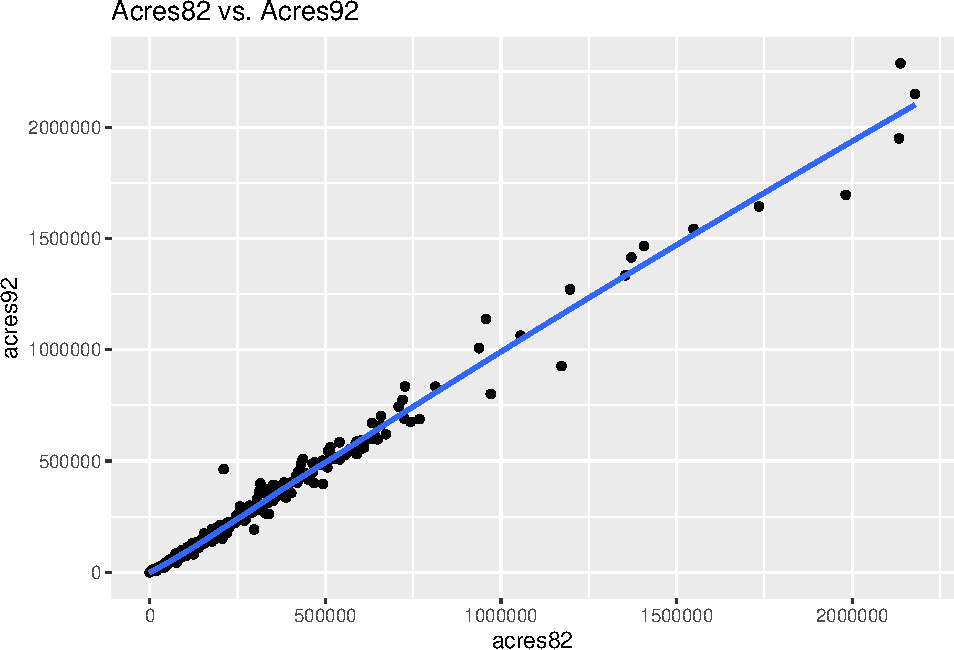
\includegraphics{homework4_files/figure-latex/unnamed-chunk-4-1.pdf} As
we can see from the graph, while the two lines are very similar, they
are still slightly different lines and do not completely coincide.

\hypertarget{c}{%
\subsubsection{(2c)}\label{c}}

Do the following test: \(H_0: \beta_2 = \beta_3\)
vs.~\(H_A: \beta_2 \neq \beta_3\) where \(\beta_2\) is the coefficient
for the non-echo locating bats and \(\beta_3\) is the coefficient for
the non-echo locating birds. Report the test stat and p-value for this
test, then state your conclusion in context - carefully explaining what
these hypotheses are stating about your model for log energy.

\begin{Shaded}
\begin{Highlighting}[]
\SpecialCharTok{\textgreater{}}\NormalTok{ case1002\_lm }\OtherTok{\textless{}{-}} \FunctionTok{lm}\NormalTok{(}\FunctionTok{log}\NormalTok{(Energy) }\SpecialCharTok{\textasciitilde{}} \FunctionTok{log}\NormalTok{(Mass) }\SpecialCharTok{+}\NormalTok{ Type, }\AttributeTok{data=}\NormalTok{case1002)}
\SpecialCharTok{\textgreater{}} \FunctionTok{vcov}\NormalTok{(case1002\_lm)}
\NormalTok{                            (Intercept)    }\FunctionTok{log}\NormalTok{(Mass) Typenon}\SpecialCharTok{{-}}\NormalTok{echolocating bats}
\NormalTok{(Intercept)                 }\FloatTok{0.022460721} \SpecialCharTok{{-}}\FloatTok{0.005235301}               \FloatTok{0.009482580}
\FunctionTok{log}\NormalTok{(Mass)                  }\SpecialCharTok{{-}}\FloatTok{0.005235301}  \FloatTok{0.001983939}              \SpecialCharTok{{-}}\FloatTok{0.006869742}
\NormalTok{Typenon}\SpecialCharTok{{-}}\NormalTok{echolocating bats   }\FloatTok{0.009482580} \SpecialCharTok{{-}}\FloatTok{0.006869742}               \FloatTok{0.041078883}
\NormalTok{Typenon}\SpecialCharTok{{-}}\NormalTok{echolocating birds  }\FloatTok{0.004914868} \SpecialCharTok{{-}}\FloatTok{0.005138789}               \FloatTok{0.026439562}
\NormalTok{                           Typenon}\SpecialCharTok{{-}}\NormalTok{echolocating birds}
\NormalTok{(Intercept)                               }\FloatTok{0.004914868}
\FunctionTok{log}\NormalTok{(Mass)                                }\SpecialCharTok{{-}}\FloatTok{0.005138789}
\NormalTok{Typenon}\SpecialCharTok{{-}}\NormalTok{echolocating bats                 }\FloatTok{0.026439562}
\NormalTok{Typenon}\SpecialCharTok{{-}}\NormalTok{echolocating birds                }\FloatTok{0.024837918}
\SpecialCharTok{\textgreater{}}\NormalTok{ est }\OtherTok{\textless{}{-}}  \SpecialCharTok{{-}}\FloatTok{0.07866} \SpecialCharTok{{-}} \FloatTok{0.0235982}
\SpecialCharTok{\textgreater{}}\NormalTok{ se.est }\OtherTok{\textless{}{-}} \FunctionTok{sqrt}\NormalTok{(}\FloatTok{0.009482580}  \SpecialCharTok{+} \FloatTok{0.009482580} \SpecialCharTok{*}\NormalTok{(}\SpecialCharTok{{-}}\DecValTok{1}\NormalTok{)}\SpecialCharTok{\^{}}\DecValTok{2} \SpecialCharTok{+} \DecValTok{2}\SpecialCharTok{*}\NormalTok{(}\SpecialCharTok{{-}}\DecValTok{1}\NormalTok{)}\SpecialCharTok{*}\FloatTok{0.004914868}\NormalTok{)}
\SpecialCharTok{\textgreater{}}\NormalTok{ tstat }\OtherTok{\textless{}{-}}\NormalTok{ est}\SpecialCharTok{/}\NormalTok{se.est}
\SpecialCharTok{\textgreater{}} \DecValTok{2}\SpecialCharTok{*}\FunctionTok{pt}\NormalTok{(}\SpecialCharTok{{-}}\NormalTok{tstat, }\AttributeTok{df =} \DecValTok{18}\NormalTok{)}
\NormalTok{[}\DecValTok{1}\NormalTok{] }\FloatTok{1.701188}
\end{Highlighting}
\end{Shaded}

From the calculations shown above we get a t-stat value of -1.070 and a
corresponding p-value of 1.701. Since our p-value is much larger than
0.05, we fail to reject the alternative hypothesis and accept the null
hypothesis. As such, we cannot conclude that the effect of body weight
on mean total energy expenditure differs between non-echo locating bats
and non-echo locating birds.

\hypertarget{d}{%
\subsubsection{(2d)}\label{d}}

Draw a scatterplot of the data for this problem (colored by animal type)
and add the parallel regression lines to the plot for each type of
animal. \textbf{Hint:} See the Stat 230 Notes
\href{https://kstclair.github.io/stat-230-notes/mlr.html\#mlr-penguins1}{Section
3.4.1.1 example} for the correct way to draw a parallel line model in
\texttt{ggplot2}.

\begin{Shaded}
\begin{Highlighting}[]
\SpecialCharTok{\textgreater{}} \FunctionTok{library}\NormalTok{(skimr)}
\SpecialCharTok{\textgreater{}} \FunctionTok{skim}\NormalTok{(case1002)}
\end{Highlighting}
\end{Shaded}

\begin{longtable}[]{@{}ll@{}}
\caption{Data summary}\tabularnewline
\toprule
& \\
\midrule
\endfirsthead
\toprule
& \\
\midrule
\endhead
Name & case1002 \\
Number of rows & 20 \\
Number of columns & 3 \\
\_\_\_\_\_\_\_\_\_\_\_\_\_\_\_\_\_\_\_\_\_\_\_ & \\
Column type frequency: & \\
factor & 1 \\
numeric & 2 \\
\_\_\_\_\_\_\_\_\_\_\_\_\_\_\_\_\_\_\_\_\_\_\_\_ & \\
Group variables & None \\
\bottomrule
\end{longtable}

\textbf{Variable type: factor}

\begin{longtable}[]{@{}lrrlrl@{}}
\toprule
skim\_variable & n\_missing & complete\_rate & ordered & n\_unique &
top\_counts \\
\midrule
\endhead
Type & 0 & 1 & FALSE & 3 & non: 12, ech: 4, non: 4 \\
\bottomrule
\end{longtable}

\textbf{Variable type: numeric}

\begin{longtable}[]{@{}lrrrrrrrrrl@{}}
\toprule
skim\_variable & n\_missing & complete\_rate & mean & sd & p0 & p25 &
p50 & p75 & p100 & hist \\
\midrule
\endhead
Mass & 0 & 1 & 262.68 & 220.9 & 6.70 & 63.35 & 266.5 & 391.00 & 779.0 &
▇▃▅▁▂ \\
Energy & 0 & 1 & 19.52 & 14.0 & 1.02 & 7.61 & 22.6 & 28.23 & 43.7 &
▇▂▆▅▂ \\
\bottomrule
\end{longtable}

\begin{Shaded}
\begin{Highlighting}[]
\SpecialCharTok{\textgreater{}}\NormalTok{ case1002\_lm }\OtherTok{\textless{}{-}} \FunctionTok{lm}\NormalTok{(}\FunctionTok{log}\NormalTok{(Energy) }\SpecialCharTok{\textasciitilde{}} \FunctionTok{log}\NormalTok{(Mass) }\SpecialCharTok{+}\NormalTok{ Type, }\AttributeTok{data=}\NormalTok{case1002)}
\SpecialCharTok{\textgreater{}} \FunctionTok{kable}\NormalTok{(}\FunctionTok{tidy}\NormalTok{(case1002\_lm))}
\end{Highlighting}
\end{Shaded}

\begin{longtable}[]{@{}lrrrr@{}}
\toprule
term & estimate & std.error & statistic & p.value \\
\midrule
\endhead
(Intercept) & -1.4976965 & 0.1498690 & -9.9933702 & 0.0000000 \\
log(Mass) & 0.8149575 & 0.0445414 & 18.2966182 & 0.0000000 \\
Typenon-echolocating bats & -0.0786637 & 0.2026793 & -0.3881190 &
0.7030432 \\
Typenon-echolocating birds & 0.0235982 & 0.1576005 & 0.1497345 &
0.8828453 \\
\bottomrule
\end{longtable}

\begin{Shaded}
\begin{Highlighting}[]
\SpecialCharTok{\textgreater{}}\NormalTok{ case1002\_augment }\OtherTok{\textless{}{-}} \FunctionTok{augment}\NormalTok{(case1002\_lm)  }\CommentTok{\# add fitted values}
\SpecialCharTok{\textgreater{}} \FunctionTok{ggplot}\NormalTok{(case1002\_augment, }\FunctionTok{aes}\NormalTok{(}\StringTok{\textasciigrave{}}\AttributeTok{log(Mass)}\StringTok{\textasciigrave{}}\NormalTok{, }\StringTok{\textasciigrave{}}\AttributeTok{log(Energy)}\StringTok{\textasciigrave{}}\NormalTok{, }\AttributeTok{color =}\NormalTok{ Type)) }\SpecialCharTok{+} 
\SpecialCharTok{+}   \FunctionTok{geom\_point}\NormalTok{() }\SpecialCharTok{+} 
\SpecialCharTok{+}   \FunctionTok{geom\_smooth}\NormalTok{(}\AttributeTok{se =} \ConstantTok{FALSE}\NormalTok{)}\SpecialCharTok{+} 
\SpecialCharTok{+}   \FunctionTok{geom\_line}\NormalTok{(}\FunctionTok{aes}\NormalTok{(}\AttributeTok{y =}\NormalTok{ .fitted), }\AttributeTok{size =} \DecValTok{1}\NormalTok{)}
\StringTok{\textasciigrave{}}\AttributeTok{geom\_smooth()}\StringTok{\textasciigrave{}}\NormalTok{ using method }\OtherTok{=} \StringTok{\textquotesingle{}loess\textquotesingle{}}\NormalTok{ and formula }\StringTok{\textquotesingle{}y \textasciitilde{} x\textquotesingle{}}
\NormalTok{Warning }\ControlFlowTok{in} \FunctionTok{simpleLoess}\NormalTok{(y, x, w, span, }\AttributeTok{degree =}\NormalTok{ degree, }\AttributeTok{parametric =}
\NormalTok{parametric, }\SpecialCharTok{:}\NormalTok{ span too small. fewer data values than degrees of freedom.}
\NormalTok{Warning }\ControlFlowTok{in} \FunctionTok{simpleLoess}\NormalTok{(y, x, w, span, }\AttributeTok{degree =}\NormalTok{ degree, }\AttributeTok{parametric =}
\NormalTok{parametric, }\SpecialCharTok{:}\NormalTok{ pseudoinverse used at }\FloatTok{1.889}
\NormalTok{Warning }\ControlFlowTok{in} \FunctionTok{simpleLoess}\NormalTok{(y, x, w, span, }\AttributeTok{degree =}\NormalTok{ degree, }\AttributeTok{parametric =}
\NormalTok{parametric, }\SpecialCharTok{:}\NormalTok{ neighborhood radius }\FloatTok{0.19049}
\NormalTok{Warning }\ControlFlowTok{in} \FunctionTok{simpleLoess}\NormalTok{(y, x, w, span, }\AttributeTok{degree =}\NormalTok{ degree, }\AttributeTok{parametric =}
\NormalTok{parametric, }\SpecialCharTok{:}\NormalTok{ reciprocal condition number }\DecValTok{0}
\NormalTok{Warning }\ControlFlowTok{in} \FunctionTok{simpleLoess}\NormalTok{(y, x, w, span, }\AttributeTok{degree =}\NormalTok{ degree, }\AttributeTok{parametric =}
\NormalTok{parametric, }\SpecialCharTok{:}\NormalTok{ There are other near singularities as well. }\FloatTok{6.2727}
\NormalTok{Warning }\ControlFlowTok{in} \FunctionTok{simpleLoess}\NormalTok{(y, x, w, span, }\AttributeTok{degree =}\NormalTok{ degree, }\AttributeTok{parametric =}
\NormalTok{parametric, }\SpecialCharTok{:}\NormalTok{ span too small. fewer data values than degrees of freedom.}
\NormalTok{Warning }\ControlFlowTok{in} \FunctionTok{simpleLoess}\NormalTok{(y, x, w, span, }\AttributeTok{degree =}\NormalTok{ degree, }\AttributeTok{parametric =}
\NormalTok{parametric, }\SpecialCharTok{:}\NormalTok{ pseudoinverse used at }\FloatTok{5.5474}
\NormalTok{Warning }\ControlFlowTok{in} \FunctionTok{simpleLoess}\NormalTok{(y, x, w, span, }\AttributeTok{degree =}\NormalTok{ degree, }\AttributeTok{parametric =}
\NormalTok{parametric, }\SpecialCharTok{:}\NormalTok{ neighborhood radius }\FloatTok{0.89511}
\NormalTok{Warning }\ControlFlowTok{in} \FunctionTok{simpleLoess}\NormalTok{(y, x, w, span, }\AttributeTok{degree =}\NormalTok{ degree, }\AttributeTok{parametric =}
\NormalTok{parametric, }\SpecialCharTok{:}\NormalTok{ reciprocal condition number }\DecValTok{0}
\NormalTok{Warning }\ControlFlowTok{in} \FunctionTok{simpleLoess}\NormalTok{(y, x, w, span, }\AttributeTok{degree =}\NormalTok{ degree, }\AttributeTok{parametric =}
\NormalTok{parametric, }\SpecialCharTok{:}\NormalTok{ There are other near singularities as well. }\FloatTok{0.82985}
\end{Highlighting}
\end{Shaded}

\includegraphics{homework4_files/figure-latex/unnamed-chunk-6-1.pdf}

\begin{center}\rule{0.5\linewidth}{0.5pt}\end{center}

\hypertarget{problem-3-agstrat-data-revisited-again}{%
\subsection{Problem 3: Agstrat data revisited
again}\label{problem-3-agstrat-data-revisited-again}}

Recall the \texttt{agstrat.csv} data used for homework 1 and 2. This was
a stratified random sample of US counties. We will consider the
regression of farm acreage in 1992 (y) on farm acreage in 1982 (x).

\begin{Shaded}
\begin{Highlighting}[]
\SpecialCharTok{\textgreater{}}\NormalTok{ agstrat }\OtherTok{\textless{}{-}} \FunctionTok{read.csv}\NormalTok{(}\StringTok{"http://people.carleton.edu/\textasciitilde{}kstclair/data/agstrat.csv"}\NormalTok{)}
\end{Highlighting}
\end{Shaded}

\hypertarget{a-1}{%
\subsubsection{(3a)}\label{a-1}}

Fit the regression of the \texttt{log} of \texttt{acres92} on the
\texttt{log} of \texttt{acres82} and \texttt{region} with rows 119 (New
York County, NY) and 168 (Parish County, LA) removed from the data.
(These counties have very low or 0 acres). Write down the fitted mean
functions (models) for each of the four regions. Simplify your
models/equations as much as possible (e.g.~give a formula with estimated
slope and intercept for each of the regions, but no need to ``unlog''
your variables.)

\begin{Shaded}
\begin{Highlighting}[]
\SpecialCharTok{\textgreater{}}\NormalTok{ agstrat\_new }\OtherTok{\textless{}{-}}\NormalTok{ agstrat }\SpecialCharTok{\%\textgreater{}\%} \FunctionTok{slice}\NormalTok{(}\SpecialCharTok{{-}}\DecValTok{119}\NormalTok{,}\SpecialCharTok{{-}}\DecValTok{168}\NormalTok{)}
\SpecialCharTok{\textgreater{}}\NormalTok{ agstrat }\OtherTok{\textless{}{-}} \FunctionTok{read.csv}\NormalTok{(}\StringTok{"http://people.carleton.edu/\textasciitilde{}kstclair/data/agstrat.csv"}\NormalTok{)}
\SpecialCharTok{\textgreater{}}\NormalTok{ agstrat\_new }\OtherTok{\textless{}{-}}\NormalTok{ agstrat }\SpecialCharTok{\%\textgreater{}\%} \FunctionTok{slice}\NormalTok{(}\SpecialCharTok{{-}}\DecValTok{119}\NormalTok{,}\SpecialCharTok{{-}}\DecValTok{168}\NormalTok{)}
\SpecialCharTok{\textgreater{}}\NormalTok{ agstrat\_lm }\OtherTok{\textless{}{-}} \FunctionTok{lm}\NormalTok{(}\FunctionTok{log}\NormalTok{(acres92) }\SpecialCharTok{\textasciitilde{}} \FunctionTok{log}\NormalTok{(acres82) }\SpecialCharTok{+}\NormalTok{ region, }\AttributeTok{data =}\NormalTok{ agstrat\_new)}
\SpecialCharTok{\textgreater{}} \FunctionTok{kable}\NormalTok{(}\FunctionTok{tidy}\NormalTok{(agstrat\_lm))}
\end{Highlighting}
\end{Shaded}

\begin{longtable}[]{@{}lrrrr@{}}
\toprule
term & estimate & std.error & statistic & p.value \\
\midrule
\endhead
(Intercept) & -0.7251775 & 0.1061376 & -6.8324272 & 0.0000000 \\
log(acres82) & 1.0539321 & 0.0084236 & 125.1165159 & 0.0000000 \\
regionNE & -0.0920789 & 0.0352412 & -2.6128212 & 0.0094432 \\
regionS & -0.0126336 & 0.0190963 & -0.6615755 & 0.5087632 \\
regionW & -0.0248363 & 0.0258738 & -0.9599040 & 0.3378950 \\
\bottomrule
\end{longtable}

\begin{Shaded}
\begin{Highlighting}[]
\SpecialCharTok{\textgreater{}}\NormalTok{ agstrat\_augment }\OtherTok{\textless{}{-}} \FunctionTok{augment}\NormalTok{(agstrat\_lm)  }\CommentTok{\# add fitted values}
\SpecialCharTok{\textgreater{}} \FunctionTok{ggplot}\NormalTok{(agstrat\_augment, }\FunctionTok{aes}\NormalTok{(}\StringTok{\textasciigrave{}}\AttributeTok{log(acres92)}\StringTok{\textasciigrave{}}\NormalTok{, }\StringTok{\textasciigrave{}}\AttributeTok{log(acres82)}\StringTok{\textasciigrave{}}\NormalTok{, }\AttributeTok{color =}\NormalTok{ region)) }\SpecialCharTok{+} 
\SpecialCharTok{+}   \FunctionTok{geom\_point}\NormalTok{() }\SpecialCharTok{+} 
\SpecialCharTok{+}   \FunctionTok{geom\_smooth}\NormalTok{(}\AttributeTok{se =} \ConstantTok{FALSE}\NormalTok{) }\SpecialCharTok{+} 
\SpecialCharTok{+}   \FunctionTok{geom\_line}\NormalTok{(}\FunctionTok{aes}\NormalTok{(}\AttributeTok{y =}\NormalTok{ .fitted), }\AttributeTok{size =} \DecValTok{1}\NormalTok{)}
\StringTok{\textasciigrave{}}\AttributeTok{geom\_smooth()}\StringTok{\textasciigrave{}}\NormalTok{ using method }\OtherTok{=} \StringTok{\textquotesingle{}loess\textquotesingle{}}\NormalTok{ and formula }\StringTok{\textquotesingle{}y \textasciitilde{} x\textquotesingle{}}
\end{Highlighting}
\end{Shaded}

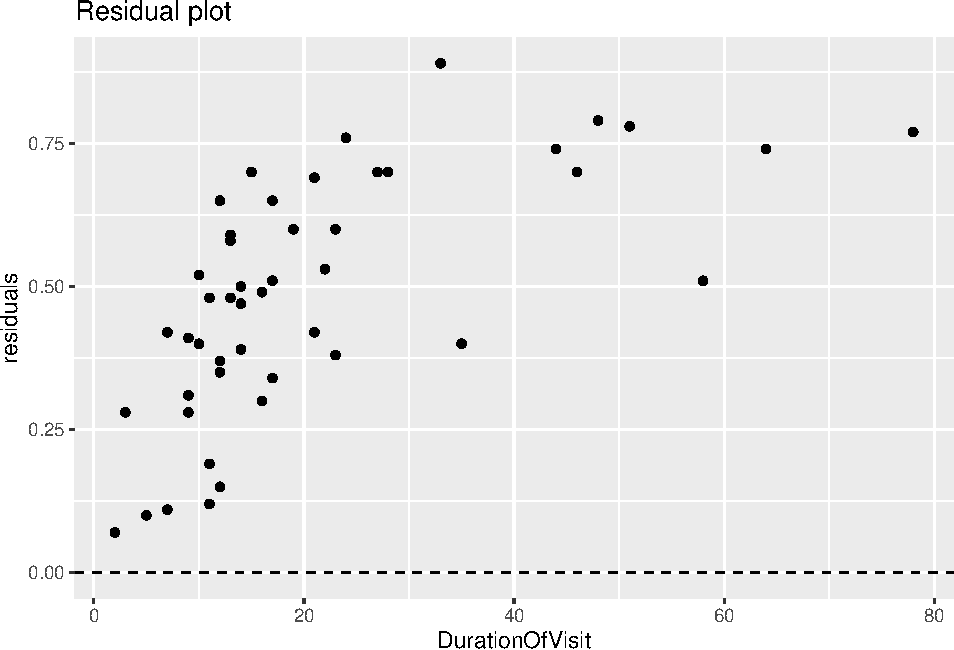
\includegraphics{homework4_files/figure-latex/unnamed-chunk-8-1.pdf}

\begin{Shaded}
\begin{Highlighting}[]
\SpecialCharTok{\textgreater{}} \FunctionTok{glance}\NormalTok{(agstrat\_lm) }\SpecialCharTok{\%\textgreater{}\%} \FunctionTok{select}\NormalTok{(df.residual, nobs) }\SpecialCharTok{\%\textgreater{}\%} \FunctionTok{kable}\NormalTok{()}
\end{Highlighting}
\end{Shaded}

\begin{longtable}[]{@{}rr@{}}
\toprule
df.residual & nobs \\
\midrule
\endhead
293 & 298 \\
\bottomrule
\end{longtable}

\[
\hat \mu_{log(acres92)|log(acres82), region} = -0.7251775 + 1.0539321(log(acres82)) - 0.0920789(regionNE) - 0.0126336(regionS) - 0.0248363(regionW)
\] \[
\hat \mu_{log(acres92)|log(acres82), region = NC} = -0.7251775 + 1.0539321(log(acres82)) - 0.0920789(0) - 0.0126336(0) - 0.0248363(0) = -0.7251775 + 1.0539321(log(acres82))
\] \[
\hat \mu_{log(acres92)|log(acres82), region = NE} = -0.7251775 + 1.0539321(log(acres82)) - 0.0920789(1) - 0.0126336(0) - 0.0248363(0) = 0.7251775 + 1.0539321(log(acres82)) - 0.0920789
\] \[
\hat \mu_{log(acres92)|log(acres82), region = S} = -0.7251775 + 1.0539321(log(acres82)) - 0.0920789(0) - 0.0126336(1) - 0.0248363(0) = 0.7251775 + 1.0539321(log(acres82)) - 0.0126336
\] \[
\hat \mu_{log(acres92)|log(acres82), region = W} = -0.7251775 + 1.0539321(log(acres82)) - 0.0920789(0) - 0.0126336(0) - 0.0248363(1) = 0.7251775 + 1.0539321(log(acres82)) - 0.0248363
\] Note: you can omit one or more cases from a \texttt{lm} by adding a
\texttt{subset} argument to the command. For example, adding
\texttt{subset=-c(119,168)} to the \texttt{lm} command will omit rows
119 and 168 from your regression fit!

\hypertarget{b-1}{%
\subsubsection{(3b)}\label{b-1}}

Consider the t-test for the parameter \(\beta_{NE}\) (the \(\beta\)
parameter for the NE region). Using the p-value given for the t-test,
carefully interpret the result of this test.

\[
t-test = \frac{-0.0920789 - 0}{0.0352412} = -2.61282
\]

\[
2*pt(2.61282, df=293) = 1.990557
\] From the calculations shown above we get a t-stat value of -2.61282
and a corresponding p-value of 1.990557 Since our p-value is much larger
than 0.05, we fail to reject the alternative hypothesis and accept the
null hypothesis. As such, we cannot conclude that there is an effect of
acreage in 82 in the NE region on mean acreage in 92 in the NE region,
after controlling all other variables.

\begin{center}\rule{0.5\linewidth}{0.5pt}\end{center}

\hypertarget{problem-4-wages-and-race}{%
\subsection{Problem 4: Wages and Race}\label{problem-4-wages-and-race}}

Consider ch.10 exercise 29 to answer the following questions. Review the
background info for this exercise and data coding provided by the
exercise description. We will still consider whether the CPS provides
evidence of racial discrimination with respect to wages after accounting
for factors like education, experience and location. Here is the model
we are considering for this problem: \[
\mu(\log(WeeklyEarnings)) = \beta_0 + \beta_1 Educ + \beta_2 Exper + \beta_3 RaceNotBlack + \beta_4 MetStatus + \beta_5 regionNE +\beta_6 regionS + \beta_7 regionW + \beta_8 regionNE \times RaceNotBlack +\beta_9 regionS \times RaceNotBlack+ \beta_{10} regionW\times RaceNotBlack
\]

\hypertarget{a-2}{%
\subsubsection{(4a)}\label{a-2}}

Write down the model mean function for Black males in the midwest
region. Then repeat this for non-Black males in the midwest. Which
\textbf{one} parameter (\(\beta\)) measures the difference in mean
earnings between Black and non-Black populations in the midwest region?

\[
\mu(\log(WeeklyEarnings)|black, region = MW) = \beta_0 + \beta_1 Educ + \beta_2 Exper + \beta_4 MetStatus
\]

\[
\mu(\log(WeeklyEarnings)|notblack, region = MW) = \beta_0 + \beta_1 Educ + \beta_2 Exper + \beta_3 RaceNotBlack + \beta_4 MetStatus
\] \[
\mu(\log(WeeklyEarnings)|notblack, region = MW) - \mu(\log(WeeklyEarnings)|black, region = MW) = \beta_0 + \beta_1 Educ + \beta_2 Exper + \beta_3 RaceNotBlack + \beta_4 MetStatus - (\beta_0 + \beta_1 Educ + \beta_2 Exper + \beta_4 MetStatus) = \beta_3 RaceNotBlack
\] By subtracting the two, we see that it is the \(\beta_{3}\) that
measures the difference in mean earnings between Black and non-Black
populations in the midwest region.

\hypertarget{b-2}{%
\subsubsection{(4b)}\label{b-2}}

Write down the model mean function for Black males in the northeast
region. Then repeat this for non-Black males in the northeast. Which
\textbf{combination} of parameters (\(\beta\)'s) measures the difference
in mean earnings between Black and non-Black populations in the
northeast region?

\[
\mu(\log(WeeklyEarnings)|black, region = NE) = \beta_0 + \beta_1 Educ + \beta_2 Exper + \beta_4 MetStatus + \beta_5 regionNE +  \beta_8 regionNE \times RaceNotBlack
\]

\[
\mu(\log(WeeklyEarnings)|nonblack, region = NE) = \beta_0 + \beta_1 Educ + \beta_2 Exper + \beta_3 RaceNotBlack + \beta_4 MetStatus + \beta_5 regionNE +  \beta_8 regionNE \times RaceNotBlack
\] \[
\mu(\log(WeeklyEarnings)|nonblack, region = NE) - \mu(\log(WeeklyEarnings)|black, region = NE) =  \beta_0 + \beta_1 Educ + \beta_2 Exper + \beta_3 RaceNotBlack + \beta_4 MetStatus + \beta_5 regionNE +  \beta_8 regionNE \times RaceNotBlack - ( \beta_0 + \beta_1 Educ + \beta_2 Exper + \beta_4 MetStatus + \beta_5 regionNE +  \beta_8 regionNE \times RaceNotBlack) = \beta_3 RaceNotBlack + \beta_8 regionNE \times RaceNotBlack
\]

\hypertarget{c-1}{%
\subsubsection{(4c)}\label{c-1}}

Researchers are particularly interested in determining if the effect of
race (Black/non-Black) on earnings of males differs by region, after
controlling for region, education, experience, and metropolitan status.
Explain why the model above can be used to answer this question.

\hypertarget{d-1}{%
\subsubsection{(4d)}\label{d-1}}

Using the data for exercise 29 (\texttt{ex1029}), create the
\texttt{ggplot2} package boxplot of log earnings vs.~race \emph{faceted}
by region (make sure to turn \texttt{eval=TRUE} in your homework):

\begin{Shaded}
\begin{Highlighting}[]
\SpecialCharTok{\textgreater{}}\NormalTok{ ex1029 }\OtherTok{\textless{}{-}}\NormalTok{ ex1029}
\SpecialCharTok{\textgreater{}} \FunctionTok{ggplot}\NormalTok{(ex1029, }\FunctionTok{aes}\NormalTok{(}\AttributeTok{x=}\NormalTok{Race, }\AttributeTok{y=}\NormalTok{WeeklyEarnings)) }\SpecialCharTok{+} 
\SpecialCharTok{+}   \FunctionTok{geom\_boxplot}\NormalTok{() }\SpecialCharTok{+} 
\SpecialCharTok{+}   \FunctionTok{facet\_wrap}\NormalTok{(}\SpecialCharTok{\textasciitilde{}}\NormalTok{Region) }\SpecialCharTok{+} 
\SpecialCharTok{+}   \FunctionTok{scale\_y\_log10}\NormalTok{()}
\end{Highlighting}
\end{Shaded}

Explain what this plot shows about the relationship between earnings,
race and region. Does it support the idea that the effect of race on
earnings differs by region?

(note: you will actually fit this model and analyze it in HW 5!)

\begin{center}\rule{0.5\linewidth}{0.5pt}\end{center}

\hypertarget{problem-5-woodpecker-nesting}{%
\subsection{Problem 5: Woodpecker
nesting}\label{problem-5-woodpecker-nesting}}

\textbf{No R work is needed (expect for qt command) - all the info for
this problem is given below.} Recall the woodpecker example from the day
3 notes. Below is the output for the regression of nest depth (cm) on
air temp (Celsius), along with covariance matrix for the coefficients.
Compute a 95\% confidence interval for the mean response
\(\mu(depth \mid temp=8)=\beta_0 + \beta_1(8)\) when temp is 8 degrees
Celsius using the facts about inference for linear combinations of
coefficients from ch.~10 (section 10.4.3). Your CI should match (except
for rounding error) the CI obtained in the day 3 notes using the
\texttt{predict} command: 15.83 to 18.94 cm.

\begin{Shaded}
\begin{Highlighting}[]
\SpecialCharTok{\textgreater{}}\NormalTok{ wpdata}\OtherTok{\textless{}{-}} \FunctionTok{read.csv}\NormalTok{(}\StringTok{"http://people.carleton.edu/\textasciitilde{}kstclair/data/woodpeckers.csv"}\NormalTok{)}
\SpecialCharTok{\textgreater{}}\NormalTok{ wood\_lm}\OtherTok{\textless{}{-}} \FunctionTok{lm}\NormalTok{(depth }\SpecialCharTok{\textasciitilde{}}\NormalTok{ temp, }\AttributeTok{data =}\NormalTok{ wpdata)}
\SpecialCharTok{\textgreater{}} \FunctionTok{summary}\NormalTok{(wood\_lm)}

\NormalTok{Call}\SpecialCharTok{:}
\FunctionTok{lm}\NormalTok{(}\AttributeTok{formula =}\NormalTok{ depth }\SpecialCharTok{\textasciitilde{}}\NormalTok{ temp, }\AttributeTok{data =}\NormalTok{ wpdata)}

\NormalTok{Residuals}\SpecialCharTok{:}
\NormalTok{    Min      1Q  Median      3Q     Max }
\SpecialCharTok{{-}}\FloatTok{2.8066} \SpecialCharTok{{-}}\FloatTok{1.3321} \SpecialCharTok{{-}}\FloatTok{0.6529}  \FloatTok{0.6811}  \FloatTok{4.8512} 

\NormalTok{Coefficients}\SpecialCharTok{:}
\NormalTok{            Estimate Std. Error t value }\FunctionTok{Pr}\NormalTok{(}\SpecialCharTok{\textgreater{}}\ErrorTok{|}\NormalTok{t}\SpecialCharTok{|}\NormalTok{)    }
\NormalTok{(Intercept) }\FloatTok{20.12228}    \FloatTok{0.94024}  \FloatTok{21.401} \FloatTok{1.11e{-}09} \SpecialCharTok{**}\ErrorTok{*}
\NormalTok{temp        }\SpecialCharTok{{-}}\FloatTok{0.34218}    \FloatTok{0.05961}  \SpecialCharTok{{-}}\FloatTok{5.741} \FloatTok{0.000188} \SpecialCharTok{**}\ErrorTok{*}
\SpecialCharTok{{-}{-}{-}}
\NormalTok{Signif. codes}\SpecialCharTok{:}  \DecValTok{0} \StringTok{\textquotesingle{}***\textquotesingle{}} \FloatTok{0.001} \StringTok{\textquotesingle{}**\textquotesingle{}} \FloatTok{0.01} \StringTok{\textquotesingle{}*\textquotesingle{}} \FloatTok{0.05} \StringTok{\textquotesingle{}.\textquotesingle{}} \FloatTok{0.1} \StringTok{\textquotesingle{} \textquotesingle{}} \DecValTok{1}

\NormalTok{Residual standard error}\SpecialCharTok{:} \FloatTok{2.335}\NormalTok{ on }\DecValTok{10}\NormalTok{ degrees of freedom}
\NormalTok{Multiple R}\SpecialCharTok{{-}}\NormalTok{squared}\SpecialCharTok{:}  \FloatTok{0.7672}\NormalTok{,    Adjusted R}\SpecialCharTok{{-}}\NormalTok{squared}\SpecialCharTok{:}  \FloatTok{0.7439} 
\NormalTok{F}\SpecialCharTok{{-}}\NormalTok{statistic}\SpecialCharTok{:} \FloatTok{32.96}\NormalTok{ on }\DecValTok{1}\NormalTok{ and }\DecValTok{10}\NormalTok{ DF,  p}\SpecialCharTok{{-}}\NormalTok{value}\SpecialCharTok{:} \FloatTok{0.0001875}
\SpecialCharTok{\textgreater{}} \FunctionTok{vcov}\NormalTok{(wood\_lm)}
\NormalTok{            (Intercept)         temp}
\NormalTok{(Intercept)  }\FloatTok{0.88406062} \SpecialCharTok{{-}}\FloatTok{0.039081046}
\NormalTok{temp        }\SpecialCharTok{{-}}\FloatTok{0.03908105}  \FloatTok{0.003552822}
\end{Highlighting}
\end{Shaded}

\begin{center}\rule{0.5\linewidth}{0.5pt}\end{center}

\hypertarget{problem-6-gender-stereotypes}{%
\subsection{Problem 6: Gender
stereotypes}\label{problem-6-gender-stereotypes}}

A 2017 \emph{Science} article studied gender stereotypes around
intellect in 5-7 year old boys and girls
(\href{http://science.sciencemag.org/content/355/6323/389}{link}). For
this problem we will look at some of the data collected for studies 3
and 4, contained in the data file \texttt{SteroTypeStudy34.csv}. For
both these studies, researchers measured subject interest in either a
game for ``smart'' people or a game for people who ``try-hard.'' The
response \texttt{interest} is a standardized measure of subject interest
in the ``smart'' games, so higher \texttt{interest} means more interest
expressed in that type of game than other study subjects. The variable
\texttt{gender} records gender (boy/girl) and \texttt{age2} groups
subjects into 5-year-old (\texttt{age5}) participants and 6- to
7-year-old (\texttt{age6and7}) participants. This mimics the use of age
in some of the paper's results.

\begin{Shaded}
\begin{Highlighting}[]
\SpecialCharTok{\textgreater{}}\NormalTok{ stereo }\OtherTok{\textless{}{-}} \FunctionTok{read.csv}\NormalTok{(}\StringTok{"http://math.carleton.edu/kstclair/data/StereoTypeStudy34.csv"}\NormalTok{)}
\end{Highlighting}
\end{Shaded}

\hypertarget{a-3}{%
\subsubsection{(6a)}\label{a-3}}

Create an EDA graph that explores whether the effect of \texttt{gender}
on \texttt{interest} level is affected by the age of the subject
(measured by \texttt{age2} \emph{not} by \texttt{age}). Explain what
your graph shows you.

\hypertarget{b-3}{%
\subsubsection{(6b)}\label{b-3}}

Determine the appropriate regression model to model \texttt{interest} as
a function of \texttt{gender} and \texttt{age2} that allows the effect
of \texttt{gender} on \texttt{interest} to differ by \texttt{age2}
group. Write down your model mean function in terms of \(\beta\)
parameters first (like was done at the start of problem 4), then fit the
model in R. Then, holding age constant, write down the estimated mean
interest level for girls and for boys.

\hypertarget{c-2}{%
\subsubsection{(6c)}\label{c-2}}

Use your model in (b) to determine if interest level in ``smart'' games
differs by gender for the 5-year old age group. Give a p-value to
support your conclusion and, if statistically significant, give and
interpret a confidence interval for the effect of gender in this age
group.

\hypertarget{d-2}{%
\subsubsection{(6d)}\label{d-2}}

Repeat (c) but for the 6 to 7-year old age group.

\end{document}
